\documentclass[preprint]{elsarticle}
\usepackage{lineno,hyperref}
\usepackage{amsmath}

\modulolinenumbers[5]

\journal{Elsevier}


\bibliographystyle{model2-names}



\begin{document}

\begin{frontmatter}

\title{Partial Encryption of Video Bit-Streams using Coupled Chaotic Maps}

%% Group authors per affiliation:
\author[fa]{Fadi Almasalha}


\author[rh]{Rogelio Hasimoto-Beltr\'an}


\author[ak]{Ashfaq A. Khokhar \corref{cor1}}
\ead{ashfaq@iit.edu}

\cortext[cor1]{Corresponding author}

\address[fa]{Applied Science Private University, Amman, Jordan.}
\address[rh]{Center for Research in Mathematics (CIMAT), Guanajuato, M\'exico.}
\address[ak]{Department of ECE, Illinois Institute of Technology, Chicago, IL.}

\begin{abstract}
Due to pervasive communication infrastructures a plethora of enabling technologies is being developed over mobile and wired networks. Among these, video streaming services over IP are the most challenging in terms of quality, real-time requirements, and security. In this paper we propose a novel scheme to efficiently secure variable length coded (VLC) multimedia bit streams such as H.264. It is based on code word error diffusion and variable size segment shuffling. The codeword diffusion and the shuffling mechanisms are based on random operations using a computationally efficient secure chaotic maps random number generator. The proposed scheme is ubiquitous to the end users and can be deployed at any node in the network. It also works on the compressed bit stream without requiring any decoding. The proposed scheme is 200\% faster, and 150\% more power efficient when compared with AES-based software full encryption schemes. Regarding security, the scheme is robust to well-known attacks in the literature such as brute force and known/chosen plaintext attacks.
\end{abstract}

\begin{keyword}
Chaotic maps \sep RTP \sep Video encoding \sep VLC \sep Huffman code 
\end{keyword}

\end{frontmatter}

\linenumbers

\section{Introduction}
Due to recent developments in the field of multimedia communications, applications such as Voice over IP (VoIP), video conferencing, e-learning and digital TV/HDTV are now part of everyday life. We are immersed in a worldwide information network where people do business online, and have access to news, bank accounts, etc., from their offices or homes. These digital commodities have some inherent risks; communication networks (wired/wireless) are vulnerable to attacks violating the user's right of privacy. It is imperative to design fast and secure systems. However, in the case of multimedia data, security demands addressing new challenges, primarily due to sheer volume of data involved, temporal dependent nature of the information, and time processing restrictions for real-time multimedia communications. The problem of security for mobile communications is further exacerbated by the limited processing power and battery life available in diverse devices, particularly handheld or mobile, for which provisioning of security may be infeasible when the complexity of related decoding operations is over the processing limit of such devices. Therefore security solutions have to be power efficient to allow longer and more number of sessions between mobile users within a single battery charging cycle. Any solution involving full encryption of the information limits itself in terms of scalability. Furthermore, it is desirable that the solution should work in the compressed domain without requiring decoding of the bit stream. In this work, we focus on the encryption of partial contents rather than encrypting the complete multimedia coded bit stream. Our solution is a novel scalable technique to secure variable length coded (VLC) bit streams aimed at minimizing the encryption complexity while preserving security. It can be implemented at any stage of the communication pipeline, that is, after the encoding process on the sending device (handheld or mobile device) or at a dedicated server handling multiple multimedia streams. 

Numerous data encryption schemes have been proposed for multimedia \\streaming applications that lower the complexity by selectively encrypting the data. Khanvilkar \textit{et al}.~\cite{Khanvilkar2006} proposed a selective encryption approach for mp3 bitstreams that partially encrypted selected fields in the mp3 header. Meyer and Gadgast~\cite{Meyer1995} proposed a selective encryption scheme for MPEG-1 bit streams. The principle data to be secured included: all the headers, $I$ frames, and $I$ blocks. They proposed a number of combinations of the above scheme to attain different levels of security. Spanos and Maples~\cite{Spanos1995}  proposed to encrypt the $I$ frames and the ISO start and end code of the MPEG stream. Tang~\cite{Tang1996} proposed an approach to use random permutation list instead of the zigzag order for mapping an 8x8 DCT block to a 1x64 block. Without the actual permutation list it would be difficult to perform the inverse DCT transform on this data. This approach yielded non-optimal compression. Liu and Eskicioglu~\cite{Liu2003} gave a comparison between the traditional and selective encryption approach, and showed that selective encryption based techniques suffer in one or more of the following points:

\renewcommand{\labelenumi}{\arabic{enumi}$)$ }
\begin{enumerate}
\item Insufficient security.
\item Decrease in the compression performance of entropy coding.
\item Insignificant computational reduction with respect to total encryption.
\item Lack of bitstream compliance.
\item Increase in key size.
\item Require compression decoding. 
\end{enumerate}

Wu and Kuo~\cite{Wu2005} proposed a scheme that performs both compression and encryption by using multiple Huffman tables in the entropy encoder. The secret key used for encryption and decryption consists of $G$ distinct Huffman coding tables. Huffman tables are then selected randomly from some public pool of Huffman tables. Wen \textit{et al}.~\cite{Jiangtao2006} proposed a binary arithmetic coding with key interval splitting. The proposed scheme is designed to achieve both compression and confidentiality by splitting the intervals according to a secret key. Jakimoski and Subbalakshmi~\cite{Jakimoski2008} gave a cryptanalysis of different multimedia encryption schemes. He showed that~\cite{Jiangtao2006}  and~\cite{Wu2005} are vulnerable to low complexity known- and/or chosen-plaintext attacks. Different than the previous codec dependent security schemes, our aim is to secure VLC coded bit streams including mp3, H.263, H.264 codec through random bit changes and by generating decoding errors that propagate as long as the resulting codewords are valid. The longer the propagation error, the more secure is the system. However several works have been proposed to minimize the effect of error propagation on subsequent codewords. In~\cite{Capocelli1992, Ferguson1984, Hemami2000, Maxted1985, Montgomery1986, Chung2002}, solutions have been investigated to overcome such errors by exploiting correlation among the codewords. A straight forward solution is to drop the corrupted sequence once it is detected, and resynchronize from the new synch position within the bit stream. The research works involving self-synchronizing codes that quickly help reestablish synchronization and thus reduce the run length of error propagation can be found in~\cite{Capocelli1992, Ferguson1984, Hemami2000, Maxted1985, Montgomery1986, Chung2002}. A more complex solution is to approximate the corrupted coefficient value from previous or/and advance values. Te-Chung and Kumar~\cite{Chung2002} have studied the dependency in inter-subband coefficient values, and showed that there exists certain correlation between coefficient of parent and child subbands of a picture. Based on the subbands coefficient relation, they have proposed a scheme to recover the lost values. The scheme divides the corrupted subband into three regions, the correctly coded region, the error propagation region and the shifted region. The scheme transmits two parameters within the compressed stream to be used at the decoder stage to reconstruct the corrupted values. These types of schemes work under the assumption of isolated bite errors for which the upcoming bit sequence can be resynchronized. For additional details on security techniques related to VLC bit streams we refer to~\cite{Kitakami2005, Maxted1985}. 

In this paper we focus our work on variable length coded (VLC) video streams. The main idea of our encryption scheme is to make the decoding of the VLC codewords in the bit stream computational infeasible in the absence of a secret key. Assuming video stream consists of packets, each packet is divided into random size segments. Within each segment, bits are randomly flipped such that the correlation present among codewords is diffused. Then all the segments are randomly shuffled. The randomness of bit flipping and shuffling of segments is based on a secure random number generator. For consecutive packets the shuffling and flipping patterns are completely different, and are chosen based on unrelated random numbers that are computationally infeasible to guess from the secret key. We realize such a robust and secure random number generator using coupled chaotic maps. Our proposed scheme is 200\% faster, and 150\% more power efficient when compared with AES based full encryption schemes, and secure against common attacks such as brute force and known/chosen plaintext attacks.

\begin{figure}[!ht]
\centering
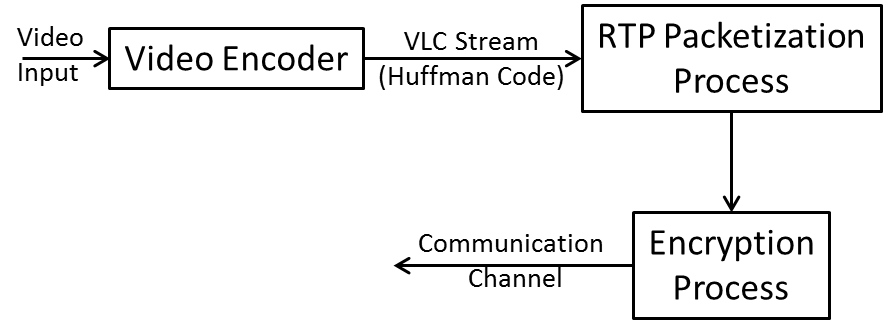
\includegraphics[width=8cm]{figure1.png}
\caption{General steps of the video data transformation process.}
\label{f1}
\end{figure}

The rest of this paper is organized as follows: In the next section we describe major components of the proposed encryption scheme. Section~\ref{SystemAnalisis} analyzes salient characteristics of the proposed scheme. In section~\ref{secSecurity}, security analysis and comparisons with existing schemes are provided.  Performance evaluation setup and experimental results are discussed in sections~\ref{evaluationSetup} and~\ref{experimentalResults}. Conclusions of the work are presented in section~\ref{conclusion}.



\section{Proposed scheme}
\label{propScheme}




The encryption process begins right after the RTP packetizing process (Figure~\ref{f1}), in which video payload (VLC bitstream) varies from 300 bytes to 1400 bytes depending on the transmitted media properties. Our proposed scheme encrypts VLC coded bitstream by performing the following dynamic operations on every RTP packet: random bit(s) flipping and segment shuffling. The position of the bits to be flipped, locations of the segments to be shuffled, and segment size depend on a secure pseudo random number generator. A block diagram of the proposed scheme is given in Figure~\ref{f2}. It is composed of three main blocks: A) Secure Random Number Generator Based on Coupled Chaotic Maps, B) Bit Flipping, and C) Segment Shuffling.

\begin{figure}[!ht]
\centering
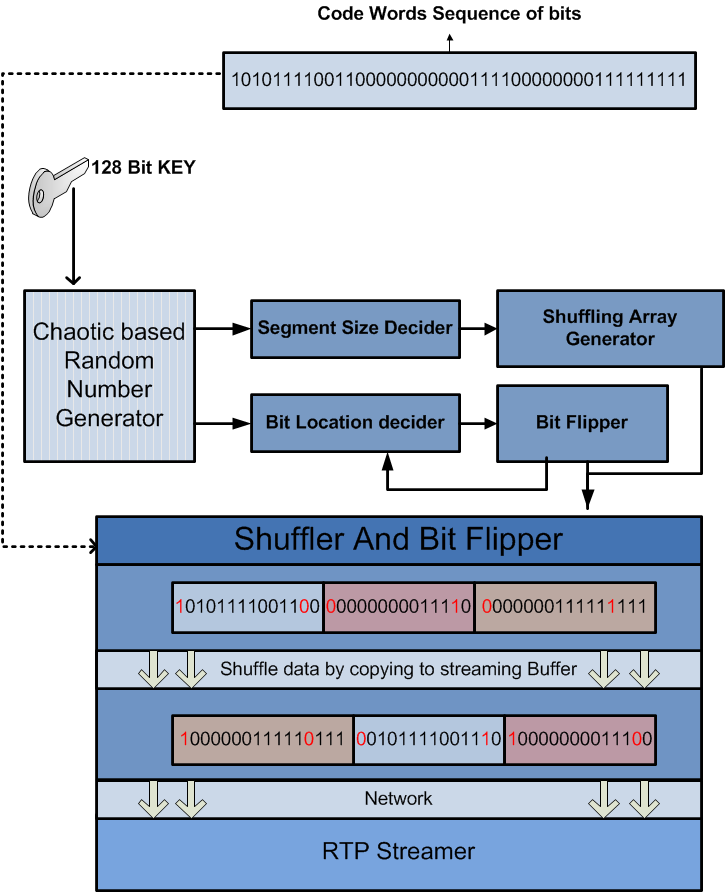
\includegraphics[width=9cm]{figure2.png}
\caption{Illustration of the proposed encryption scheme.}
\label{f2}
\end{figure}

\subsection{Secure random number generator based on chaotic maps}

The security of the proposed scheme to different attacks depends mainly on the robustness of the secure Pseudo-Random Number generator (PRNG). The scheme can work with any secure PRNG as long as the seed cannot be determined from a partially broken sequence generated. Current PRNG are not strong candidates to be included in our scheme because of their dependency on a fixed-length seed, as well as the lack of flexibility to dynamically control the security of the system. We develop a novel PRNG based on a network of $N$ chaotic maps, that is $N$ discrete chaotic maps dynamically interacting as one system but maintaining their own identity (the use of only one chaotic map does not provide enough security to the system). Discrete Chaotic Systems (DCS) have many of the good properties required in cryptography; the most prominent are sensitivity to parameters, sensitivity to initial conditions and unpredictable trajectories~\cite{Meyer1995}. The first two properties are related to diffusion, and the last one to confusion in the cryptographic nomenclature. Confusion is intended to make the relationship between cipher text and plaintext statistically independent, whereas diffusion is intended to spread out the influence of a single plaintext digit over many cipher text digits to hide the statistical structure of the plaintext. These properties have been the basis to develop secure analog and digital communication systems.

Current research in chaotic systems is focused on two main issues: \\Perturbation-based schemes and Network-based chaotic maps. Perturbation-based schemes transform stable chaotic cycles into non-stable ones by perturbing its trajectory as performed in~\cite{Meyer1995}. A network of chaotic maps or Coupled Map Lattices (CML) on the other hand considers an array of chaotic maps governed by a coupling transformation over some defined neighborhood in the array~\cite{Hasimoto2008}. In this work, we use CML to develop a PRNG that is robust to cipher text, known/chosen plaintext and differential attacks.

Our proposed PRNG is based on a network of N chaotic maps $(1 \leq i \leq N)$, represented by:

\begin{equation}
\begin{array}{c}
\displaystyle{
X_{i,j}= (1-\varepsilon)f(X_{i,j-1})+ \varepsilon H(X_{i,j-1},\; \ldots \;,X_{N,j-1 } )
}
 \\ \\
\displaystyle{
H(X_{i,j-1},\; \ldots \;,X_{N, j-1})= \sum_{i=1}^{N}w_{i}X_{i,j-1}.
}
\end{array}
\label{ec1}
\end{equation}

The states $j$ in the chaotic network represent the weighted interaction between each individual map $f(X_{i,j-1})$ (local term) and the coupling transformation $H$ (linear/nonlinear interaction term) with weights $w_{i}$, such that $\sum_{i=1}^{N}w_{i}$, and $N \geq 8$. When the weight $\varepsilon$ is weak (small magnitude), the system can be regarded as a local map perturbed by contributions from other sites, thus maintaining its main individual properties. On the other hand, when $\varepsilon$ is large, the system reaches an asymptotic collective (undesired) behavior characterized by intermittent periodic chaotic cycles (this is the case we want to avoid).

For its mathematical simplicity our selection for $f(X_{i,j})$ is the well-known logistic map represented by:

\begin{equation}
\displaystyle{
X_{i,j}= f(X_{i,j-1})= \lambda X_{i,j-1}(1-X_{i,j-1}) \; \; \; \;\; \; \lambda \in \left[ 1,4 \right) \; \;  \;\;\; \; X \in \left( 0,1 \right)
}
\label{ec2}
\end{equation}
where $\lambda$ represents the chaotic parameter and $X$ the state variable. As $\lambda$ increases from $1$ to $4$, the map experiences a period doubling to chaos. In particular for $\lambda \geq 3.5699$ (known as accumulation point) it presents a chaotic behavior, however there are many undesired periodic windows with short periods that appear abruptly. A very well-known and prominent period-3 window appears at $\lambda = 1+ \sqrt{8}= 3.8284$. Fixed points $(f(X)=X)$ are also present at $X=0$ and $X=(\lambda -1)/\lambda$, which define a regular pattern in the logistic map. In order to keep the good chaotic dynamic of the logistic map, we avoid bad initial values of $X$ and $\lambda$, and endorse the use of at least 8 chaotic maps to increase the cycle length period or the use of cycle-length tracking schemes as the one proposed in~\cite{Hasimoto2011}. It is important to point out that any chaotic map in the literature (Renyi Map, Piece-wise Linear map, etc.) can be used in Eq.~\ref{ec1}. The security relies on the scheme itself, rather than the chaotic map used in the scheme.

As mentioned before, the main reason for developing our own PRNG scheme is to manage the security of the system by creating a (near) cycle free chaotic signal capable of handling long-term multimedia communications such as VOIP and video streaming (which can last from minutes to hours). The security is controlled by changing the number of chaotic maps and periodically perturbing the system state (variables, parameters, coupling function, weight $\varepsilon$, etc.). Additionally, we include previous input data $P$ (called plaintext) as part of the coupling function $H$ to allow diffusion of the information onto the entire ciphertext output as follows:

\begin{equation}
\begin{array}{c}
\displaystyle{
H_{j}(X_{i,j},\; \ldots \; ,	X_{N,j},P)= \sum_{l=1}^{N}w_{l}X_{i,j}+ w_{N+1}\left(H'_{pkt,l}(P)\right)
} 
 \\
 \\
\displaystyle{
H'_{pkt,l}(P)=  \left(\sum_{l=1}^{M}H_{pkt-1,l} \right) \; mod \; 1
}
\end{array}
\label{ec3}
\end{equation}
where $\sum_{l=1}^{M}H_{pkt-1,l} $ represents the sum of all 32-bit coupling variables in the previous RTP packet. A bit change in $P$ affects the outcome of the bit-flipping and shuffling operations of future iterations proportionally to the magnitude of $w_{N+1}$ and $\varepsilon$. Even though the computational complexity of the scheme is slightly increased, a single plaintext change produces a totally different ciphertext, therefore increasing its robustness to statistical attacks. 

To further protect the system against security attacks, the following actions are considered:

\begin{enumerate}
\item Every iteration in Eq.~\ref{ec3} produces $N$ 32-bit chaotic trajectories (or pseudo-random numbers) coming from randomly selected chaotic maps. That is, previously evaluated chaotic map trajectory in Eq.~\ref{ec3} determines the next map to be iterated $(next\_map = previous\_chaotic\_trajectory\; mod\; N)$. In the case of an attack, the random selection of maps increases the complexity considerably.

\item The actual random number to be used in the encryption process is produced by operating three different maps according to the following formula:

\begin{equation}
Out_{i}= \left[  (X_{i,j}' + X_{i+1,j}')\; mod \;2^{PR}   \right] \oplus X_{i+2,j}'
\label{ec4}
\end{equation}
where $PR$ is the computer precision (32 or 64 bits), $\oplus$ is the XOR operator, and $X_{i,j}'$ is the integer part of $X_{i,j}$ $(X_{i,j}' =\int [X_{i,j} \ast 2^{32} ])$.

\item Only $1 \leq U \leq 27$ bits of $Out_{i}$ per map are taken into account in the encryption process; the remaining $L=U-27$ bits are used for future encryption in a randomly selected iteration. These actions prevent the attacker from having complete knowledge of the system even when the security of state variables $X_{i}'s$ has been compromised (see section~\ref{secSecurity}). Equations~\ref{ec1} -~\ref{ec4} form the Chaotic-based Random Number Generator block in Figure~\ref{f2}, and are encapsulated in function $rnd (U)$, which returns a $U$-bit random number $Out_{i}$ from the $N$ 32-bit random numbers generated.
\end{enumerate}

\begin{figure}[!ht]
\centering
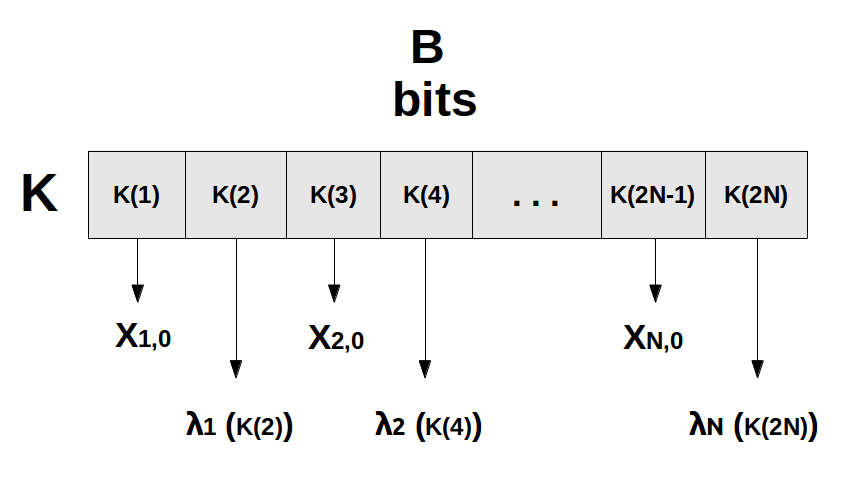
\includegraphics[width=7cm]{figure3.png}
\caption{System-key $(K)$ partition $(n/2)$ for the creation of maps variables $(X_{i},0)$ and corresponding parameters $(\lambda_{i})$.}
\label{f3}
\end{figure}


\subsubsection{Chaotic system generation}

The proposed scheme is symmetric, therefore the initial system-key $(K)$ of size $B$ bits, for $B \geq 128$ is shared between cipher and decipher. Any suitable key establishment/distribution protocol (public-key or authenticated protocol) in the literature can be used for the key exchange, the only restriction is that every session requires a new and independent system-key.

The system-key $K$ is used to initialize the $N$-array of chaotic maps as follows (see Figure \ref{f3}):

\begin{equation}
\begin{array}{l}
X_{i,0}= K_{n/2}(2i-1)/2^{n/2},
\\ \\
\displaystyle{
\lambda_{i}= 3.68+ \frac{[K_{n/2} (2i)/2^{n/2}+ K_{n/2}(2i)10^{h_{n/2}}+ (a \oplus b)/2^{n/4} ]}{10}\cdot \frac{[0.3187]}{MAX},
}
\\ \\
i = 1, 2, \; \ldots \;, N
\end{array}
\label{ec5}
\end{equation} 
where $n=B/N$ is the assigned number of bits per map (taken from $K$) for the initialization of $\lambda_{i}$ and $X_{i,0}$ ($n/2$ bits per variable and parameter) with $N \ll B$ and $(B \; mod \; N) = 0$, $K_{n/2}(m)$ represents the system-key as an array of $n/2$ bits per element, $h_{n/2}$ is the number of digits in the largest decimal number represented by $n/2$ bits, $a \oplus b$ term is the XOR between the half-most and half-least significant bits of $K_{n/2}(2i)$ respectively, yielding an $n/4$ bits outcome, and $MAX$ is the maximum value of $[K_{n/2}(2i)/2^{n/2} + K_{n/2}(2i)/10^{h_{n/2}} + (a \oplus b)/ 2^{n/4} ]/10$.


The chaotic variables and parameters are forced to fall in the range $X_{i,0} \in (0,1)$ (except $\{\lambda /(\lambda -1), 0.5\}$, which represent bad initial points) and $3.68 \leq \lambda_{i} \leq 3.998$ for $\lambda_{i} \neq \lambda_{j}$ and $i \neq j$ respectively. The remaining variables in eq.~\ref{ec1} $\varepsilon$ and $w_{i}$, $1 \leq i \leq N$ are initialized by iterating $N+1$ times a predefined map $X_{p}$ in the chaotic system. The first $N$ chaotic values are used to compute $w_{i}= X_{p,i} / \sum_{j=1}^{N}X_{p,j}$, and the last value to compute $\varepsilon= \Delta \varepsilon \cdot X_{p,N+1}+ \varepsilon _{\min}$, which represents a linear transformation from the chaotic space $X \in (0,1)$ onto the $\varepsilon \in (\varepsilon_{\min}, \varepsilon_{\max} )$  with $\Delta \varepsilon = (\varepsilon_{\max} - \varepsilon_{\min})$, $\varepsilon_{\min}$ and $\varepsilon_{\max}$ the allowable minimum and maximum value of $\varepsilon$ respectively.

\begin{table}[!ht]
\centering
\begin{tabular}{ c c c  }
\hline 
    \textbf{Key Length}   &
 \textbf{Minimum Number}&
\textbf{Maximum Number} \\ 
    \textbf{(BITS)}   &
 \textbf{of Maps $(\mathbf{MIN_{B}})$}&
\textbf{of Maps $(\mathbf{MAX_{B}})$} \\ 
\hline
\multicolumn{1}{c}{128} 	 &  \multicolumn{1}{c}{8}    &  \multicolumn{1}{c}{16}      \\ \hline
\multicolumn{1}{c}{256}   & \multicolumn{1}{c}{8}    & \multicolumn{1}{c}{25}    \\ \hline
\multicolumn{1}{c}{512}   &	\multicolumn{1}{c}{16}   &  \multicolumn{1}{c}{32}  \\
\hline 
\end{tabular}
\caption{Minimum and maximum number of chaotic maps involved in the encryption process as a function of the system-key length.
}
\label{table1}
\end{table}


After the chaotic system has been created, we perform an additional operation to increase its sensitivity to bit changes $K$ (if $K$ is changed by one bit, the new chaotic system will differ significantly from the original one). The original initial chaotic variable $X_{i,0}$ is iterated random number of times, say $R$, over the newly created coupled chaotic system, and the corresponding output becomes the initial state for each map in the encryption process. The same process can be performed for the corresponding map parameters $(\lambda_{i})$, if needed, using the new variables.

The system-key $K$ is used to define the number of chaotic maps to be used in Eq.~\ref{ec5} as follows:

\begin{equation}
\begin{array}{l @{\vrule height 12pt depth 10pt width 0pt}  }
N= \left[KS \;mod \; (MAX_{B}+1) \right],
\\ 
KS = \sum_{i=1}^{D/8}KEY_{8}(i)
\end{array}
\label{ec6}
\end{equation}
where $MIN_{B} \leq N \leq MAX_{B}$ following Table \ref{table1}.



\subsection{Bit flipping}
\label{bitfli}

Once the encryption system receives an RTP packet, the main step in our scheme is to diffuse and destroy the meaning of compressed codeword sequence and make it impractical to predict the original codeword sequence. To achieve this, we propose the flipping of at least one bit every $BF= f \cdot Av \cdot MEPL$ bits, where $Av$ is the average size of Huffman codes, $MEPL$ is the calculated Mean Average Propagation Length (MEPL) in codeword units  (described in section~\ref{SystemAnalisis}), $ Av \cdot MEPL$ is the average error propagation in bits, and $f$ is a tunable security factor with values $1/(MEPL) \leq f \leq \frac{3}{4}$. For this range of $f$, $Av \leq BF \leq (Av \cdot MEPL)$ that is, at least one bit is changed per average Huffman codeword size $(Av)$ up to $\frac{3}{4}(Av \cdot MEPL)$ bits. This is what makes \textit{our system scalable secured}, as $f$ gets smaller more bits are flipped per $BF$-bits units increasing the system security. Depending on the specific needs of the user, $f$ provides a tradeoff between security and
performance.

The actual location $B_{i}$ of the bit to be flipped in the stream is calculated as follows:

\begin{equation}
B_{i}= \left[ rnd(  \lceil   \log_{2}(f \cdot Av \cdot MEPL)  \rceil )\; mod\; BF   \right] +1
\label{ec7}
\end{equation}
where $rnd(\#bits)$ is our own designed PRNG function described in the previous section. The argument 
$\lceil   \log_{2}(f \cdot Av \cdot MEPL)  \rceil$ represents the bit-length of the requested random
number with bounds $1 \leq B_{i} \leq BF$.

The algorithm for random bit flipping in the payload $P$ of size $Ps$ bytes is outlined in the following:

\noindent \hspace*{30mm} $BF= f \cdot Av \cdot MEPL$ \\
\hspace*{30mm} \textbf{for} $i=0$ \textbf{to} $(Ps \ast 8)/BF$ \textbf{steps do} \\
\hspace*{35mm} $B_{i}=\left[ rnd(  \lceil   \log_{2}(BF)  \rceil )\; mod\; BF   \right] +1 $ \\
\hspace*{35mm} $loc = i \ast (BF)$ \\
\hspace*{35mm} $Flip(P[B_{i} + loc])$ 


\subsection{Segment shuffling}

After the bit flipping process, we permute the RTP-packet payload by performing an $L$-way shuffling. Here the payload is divided into $L$ segments which are shuffled using the algorithm described below and illustrated in Figure~\ref{f4}. The complexity of the shuffling $(L!)$ is expressed in terms of $2^{S}$, where $S$ is a user controlled variable that specifies the minimum brute force complexity required to de-shuffle the $L$ segments. $L$ is obtained as follows:

\begin{equation}
L = (rnd (\lceil \log_{2}(L_{\max}) \rceil ) \;mod  \; (L_{\max} -L_{\min})) + L_{\min}
\label{ec8}
\end{equation}
where $L_{\min}$ and $L_{\max}$ are the smallest integers satisfying  $L_{\min}! \geq 2^{S}$ (for a given user input value $S$) and $L_{\max}! \geq 2^{S}$ respectively. For each iteration (or RTP Packet) the number of segments is a random number between $20 \leq L \leq 60$ which corresponds to $60 \leq S \leq 272$ (which increases the security of the system at user's needs).

\begin{figure}[!ht]
\centering
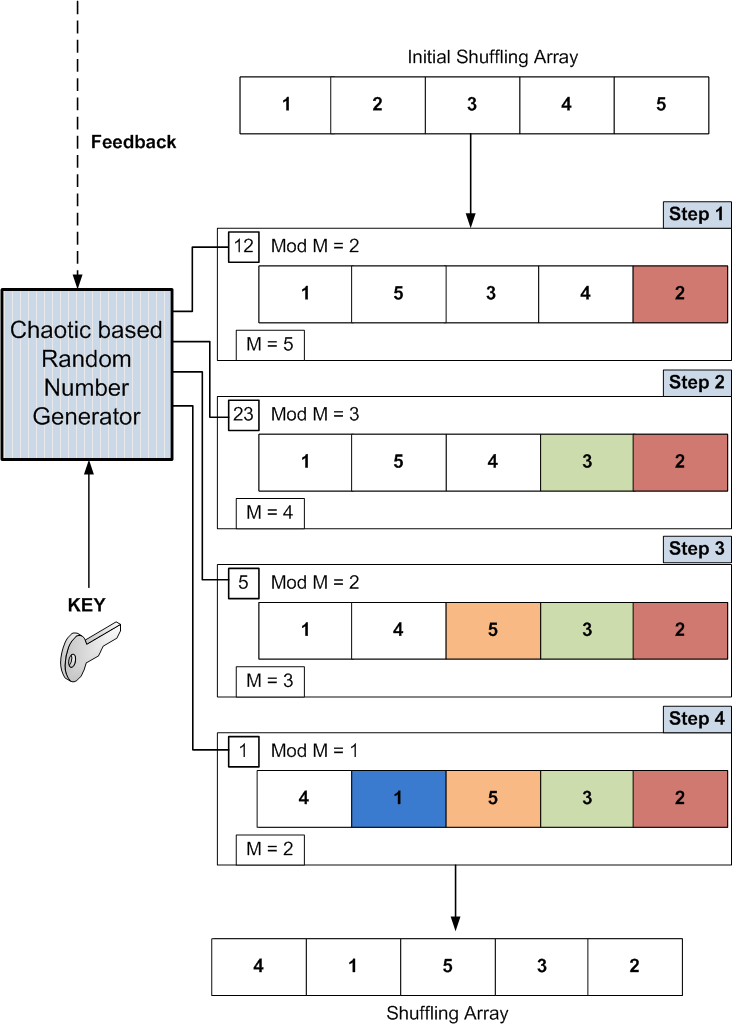
\includegraphics[width=9cm]{figure4.png}
\caption{Illustration of Building the shuffling array for an RTP packet with $L=5$ segments.}
\label{f4}
\end{figure} 

Once $L$ has been computed, the segment size $Sg$ is calculated using Eq.~\ref{ec9}:

\begin{equation}
Sg = \frac{Ps}{L}
\label{ec9}
\end{equation}
where $Ps$ is the RTP payload size in bytes. For a 300-byte RTP packet the segment size randomly falls between $5\leq Sg \leq 15$ which corresponds to $20 \leq L \leq 60$ segments.

The proposed shuffling mechanism starts by creating the shuffling array $A$ of size $L$ that will be used to shuffle the segments in $\mathcal{O}(L!)$ steps as illustrated in Figure~\ref{f4}. Each entry in the initial shuffling array is the original block index. The scheme will iterate $L-1$ times, starting by initial value of $M = L$. The following algorithm generates the shuffling array:


\noindent \hspace*{30mm} Initialize $A$ \\
\hspace*{30mm} $M=L$   \\
\hspace*{30mm} \textbf{for} $L-1$ \textbf{steps} \textbf{do} \\
\hspace*{35mm} Generate random number $R$ \\
\hspace*{35mm} $T = R\; mod \; M$ \\ 
\hspace*{35mm} Swap($A[T], A[M]$) \\
\hspace*{35mm} $M=M-1$ 


The resulted entries in array A are used to determine the new destination of each segment; the array elements are moved from current location $T$ to final location $M$ in the same array.


\section{System analysis}
\label{SystemAnalisis}

The key feature in our encryption is to make the reading and decoding of Huffman codes impossible without knowing the private key. The key characteristic exploited here is the prefix condition of the Huffman codes, which states that no code words can be a prefix of another code word~\cite{Huffman1952}.

The prefix code condition is used to guarantee the unique parsing path for each codeword, as shown in Figure~\ref{f5}. This condition provides hidden (implicit) borders that separate codeword's from each other. As we see in Figure~\ref{f5}, to satisfy the prefix code condition, each codeword ends at a leaf node in the tree. If any bit in a code word is flipped (shown with red arrow in Figure~\ref{f5}, then a transition will occur at that point which results one of the following scenarios:


\begin{figure}[!ht]
\centering
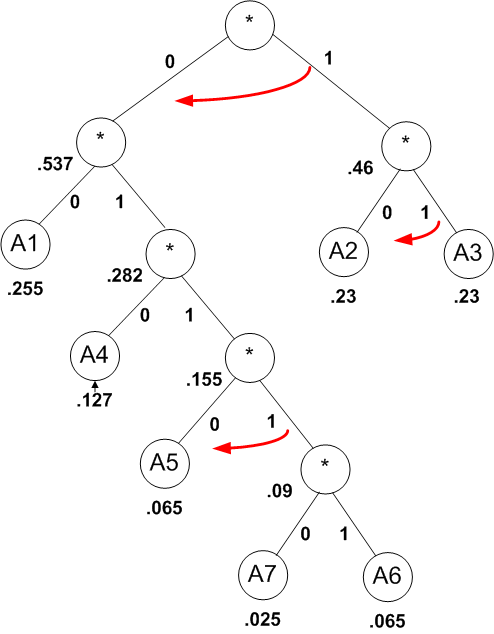
\includegraphics[width=9cm]{figure5.png}
\caption{Example of Huffman Code Tree with 3 bits flipped.}
\label{f5}
\end{figure} 

\begin{enumerate}
\item Different codeword same length size.
\item Different codeword shorter length size.
\item Different codeword longer length size.
\end{enumerate}

The first scenario will only change the codeword which includes the flipped bit. This is unlikely to happen frequently in VLC; as the length of codewords is variable. However, the effect of the corrupted codeword in this scenario on the subsequent codewords depends on the information carried out by the corrupted codeword. For example, if the codeword holds the DC value of the macroblock, the macroblock will not be decoded correctly as well as all subsequent blocks. But if the codeword holds the AC value of the macroblock, only that macroblock will not be decoded correctly. There are many candidates of what value that codeword can represent, such as DC, AC, MV, header, etc. 

\begin{figure}[!ht]
\centering
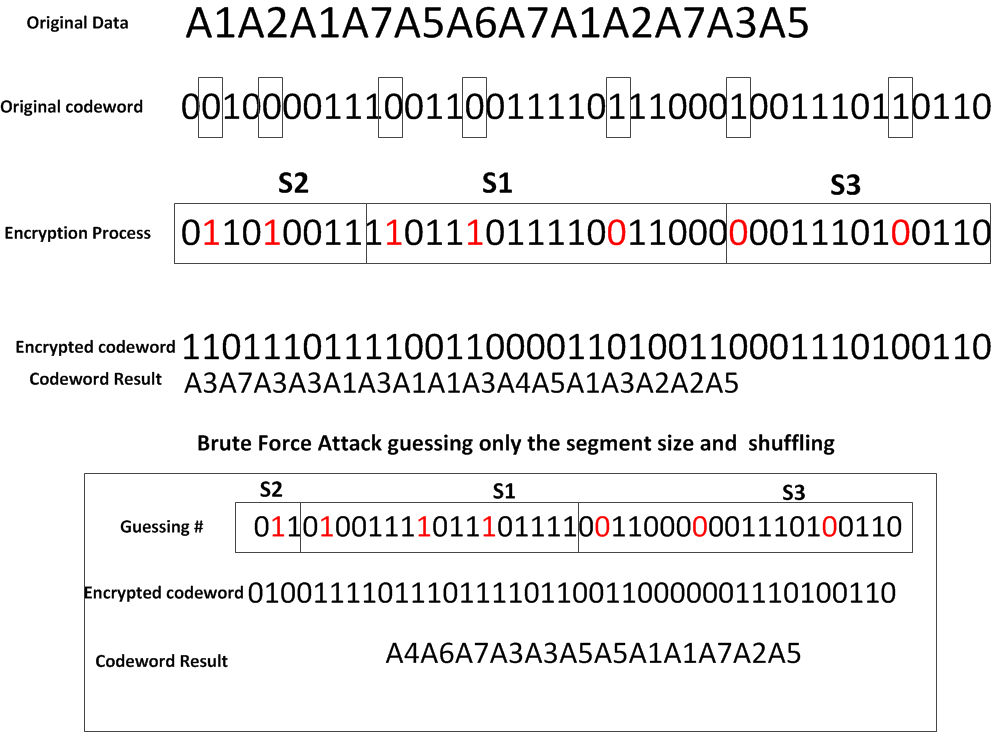
\includegraphics[width=7.7cm]{figure6.png}
\caption{Illustration of Error Propagation in Huffman codeword's.}
\label{f6}
\end{figure} 

The second and third scenarios will break the hidden borders between codewords, thus making the reading process misaligned and incorrect as shown in Figure~\ref{f6}. The error will propagate at least to the next codeword, where one of the previous scenarios can happen again. The chain of second and third scenario occurrences is called error propagation. The run length of the error propagation is at least one codeword on average. Furthermore, the mean error propagation length $MEPL$ (introduced in Section~\ref{bitfli}) for a particular bit error that occurred in a particular codeword is defined as the number of codewords in the sentence from the one where the bit error occurs to the one after which the correct parsing resumes. This concept is illustrated in Figure~\ref{f6} with an error propagation of 4 codewords. In~\cite{Monaco1987, Montgomery1986, NIST, Spanos1995, Swaszek1995} the mean error propagation length ($MEPL$) of codeword trees have been broadly studied. The concept of MEPL is also referred to as expected error span by Maxted and Robinson in~\cite{Maxted1985}. In~\cite{Maxted1985}, the authors studied an error transition model and gave a method for computing the $MEPL$. This model was further extended by Swaszek and DiCicco in~\cite{Swaszek1995}. The formulations in~\cite{Maxted1985, Monaco1987, Swaszek1995} are in algebraic forms and, as mentioned in~\cite{NIST}, a symbolic algebraic software is necessary for computing $MEPL$, especially when the code size is large. In~\cite{Takishima1994}, Takishima \textit{et al}. presented a formula for computing $MEPL$ based on crossover probability, which was further simplified to a new theorem in~\cite{Swaszek1995}. We are using the theorem in~\cite{Zhou2002} to calculate the $MEPL$ used in our encryption technique.

Our goal is to breach the prefix condition and make it unfeasible to read or guess the current or subsequent codewords. By finding the $MEPL$ value, we can approximate after how many codewords the decoder might be able to resynchronize. Thus we alter at least one bit every $\frac{3}{4} \times MEPL$ codewords and at the most one bit per codeword according to the user control security parameter $f$ (as discussed in section~\ref{bitfli}), thus forcing the decoder to be always unsynchronized. The randomness of the bit flipping operation yielding scenario (1) and scenarios (2 and 3) discussed above adds a confusion feature to the encrypted bits. This confusion makes the encryption output uncorrelated within a subsequence of codewords.




\section{Security analysis}
\label{secSecurity}
In this section we analyze the robustness of our scheme against different digital attacks, including ciphertext-only attack, known-plaintext attack, and chosen-plaintext attack. The analysis will also consider attacks for each part of our scheme: the random number generator and the shuffling/flipping bit operations. As mentioned earlier, we are using different random numbers for each shuffling/flipping operation, which eliminate the practicability of known-text attack and chosen-plaintext attack to find out the next shuffling or bit flipping operation. 



\subsection{Ciphertext-only attack:}
Cipher Text-only (Brute force) attack can target the two main components of our encryption scheme: random number generator or the bit flipping/shuffling level. First we will analyze the complexity of brute force attack on our random number generator then the bit flipping/shuffling level:


\subsubsection{Chaotic generator}
\textbf{Key space analysis}: A good cryptosystem must be sensitive to its private key, and the key space must be large enough to make a brute force attack computationally an infeasible task.  The secret key provided by the user in our scheme is assumed to be at least 128 bits, which is split into $2N$ chunks to initialize variables and parameters for the generation of the PRNG (Equations~\ref{ec1} to~\ref{ec5}).

For a 128-bit Key (see Table~\ref{table2}), we allow at least 8 bits to a maximum of 16 bits per parameter or variable in the initialization process, representing a network of 8 to 4 chaotic maps, respectively. The weights $\varepsilon$ and $w$ are obtained by iterating one of the maps a random number of times. If an attacker decides to break the system key by brute force, it will need an order of $2^{128}$ operations (just the complexity of the private key $B \geq 128$); if the attacker rather decides to brute force guessing of the variables and parameters in an $N$-map network, it will need at least $(2^{32\times N \times 2}$) operations (without considering $w_{i}$ and $\varepsilon$), which represents $2^{256}$ and $2^{512}$ operations for the minimum and maximum allowed number of maps $(N)$, respectively. 


\subsubsection{Bit flipping/shuffle}

Brute Force attack may include restoring the corrupted codewords. In this case the attacker needs to find the correct bit sequence and the correct boundary of the original stream codewords. For this to happen the attacker has to try all possible combination of bit flipping and shuffling to find the original codewords; the complete decoded frame or motion is the only guarantee of the correct order of bits and segments.

First we show the complexity to detect the location of the bit that is flipped and restore it back. Second we show the complexity to guess the shuffling order. To simplify the problem we assume that the attacker knows the average size of codewords, the $MEPL$ value and the $f$ value. Therefore he knows the range of the bit location the system flips the bits within. 

Let $V=\{v_{1},v_{2}, \ldots ,v_{J}\}$ be video stream of $J$ bits, the system flips one bit every $M \ll J$ bits and break up the stream into $R$ segments and then shuffles them. A brute force attack should perform both flipping and shuffling attack at the same time to decide which video stream is the valid one. In video compression, just decoding part of the image will not produce a valid output; the sequence of codewords is decidedly depending on previous and subsequent codewords in order to produce a valid image. Therefore, the bit flipping complexity attack for the encrypted stream for $J/M$ segments of $M$ bits can be expressed as:

\begin{equation}
\mathcal{O}(Bits \; Flipping) = M^{J/M}.
\label{ec10}
\end{equation}

On the other hand, the segment shuffling complexity attack requires the trying of all possible segment positions:

\begin{equation}
\mathcal{O}(Segment \; Shuffling) = R!.
\label{ec11}
\end{equation}

Hence the brute force complexity for both bit flipping and segment shuffling is:

\begin{equation}
\mathcal{O}(N) = R!M^{J/M}.
\label{ec12}
\end{equation}

In video transmission, the size of bit streams $J$ depends on the video properties. For example, for one $I$-Frame of $320 \times 240$ video decoded in MPEG4 format, the size will be 2Kb. The average calculated $MEPL$ value for this codec is 3, and the average codeword size is 6 bits. And let's assume that the value of $R$ is 20. Then brute force attack complexity is:

\begin{equation}
\mathcal{O}(N) = 20!6^{910}  \cong 6^{950} \cong 2^{1630}.
\label{ec13}
\end{equation}

The complexity of constructing one frame of image using brute force is a very complex task. In addition to the computation complexity, the process of recognizing a valid video output while trying bit flipping and segment shuffling requires system training and consumes a lot of computation to make decision based on the training set. This is again an extremely complex task. 

\subsection{Known-plaintext and chosen-plaintext attacks:}

In these attacks, the only candidate part to be targeted is the PRNG (chaotic generator). The bit-flipping, segmentation, and shuffling blocks are vulnerable to these attacks, but only within the same RTP packet. Successfully decoding one packet has no bearings on the next packet, as it uses different setup (bit flipping, shuffling, and segment size). Consequently, the attacker has to break down the entire chaotic system (Eq.~\ref{ec1}).  

\begin{table}[!ht]
\centering
\scalebox{0.9}{
\begin{tabular}{lllll}
\hline   
\textbf{Testbed} & \textbf{CPU} & \textbf{Clock} & \textbf{Memory} & \textbf{Operating} \\
                 & \textbf{Type} & \textbf{Speed} &                 & \textbf{System} \\
\hline
\textit{Desktop}       & 	Intel Duo Core 2   &  2.2 Ghz   &  3 GB    & Ubuntu 8.3 \\
\textit{Laptop}        & 	Intel Duo Core 2   &	  2.2 Ghz   &  2 GB    & Ubuntu 9.1   \\
\textit{NetBook}       & 	Intel Atom         &	  1.6 Ghz   &  1 GB    &  Ubuntu Netbook  \\
\textit{Nokia N800}    & 	TI Omap 2420       &	  333 Mhz   &  128 MB  &  Maemo  \\
\textit{Nokia N900}    & 	TI Omap 3430       &	  600 Mhz   &  256 MB  &  Maemo 5   \\
\hline
\end{tabular}
}
\caption{Specifications of different platforms used in experiments.}
\label{table2}
\end{table}

If we assume that the attacker has found the partial values of the chaotic variable $Out$ (least significant 27 bits used in the encryption process per map), it only knows partial information about the PRNG since $Out$ is a mask of three chaotic trajectories from three different maps. So, the next step for breaking the system is to find the remaining 5 bits of $Out$, and solve for the $X_{i}'s$ and $\lambda_{i}'s$ altogether. The attacker will need at least $2^{(N=\{4,8\}) \times (32+5)}=2^{\{148,296\}}$ operations (32 bits for the parameter $\lambda$) to tear down the second security wall given that he knows the partial values of $Out$ (this complexity is without considering $w_{i}'s$ and $\varepsilon$ in Eq.~\ref{ec1}). If we take into account that each map en Eq.~\ref{ec1} is randomly selected, the complexity of the attack increases considerably. The security of the scheme can be adjusted according to the secrecy of the ongoing multimedia communication, higher security requires increasing both the number of maps and/or the number of bits left out in the $Out$ variable. 

 
\section{Performance evaluation setup}
\label{evaluationSetup}

To evaluate the performance and power efficiency of our encryption scheme and compare it with full encryption methods, we have implemented multiple schemes on the following computing platforms: Dell desktop, Lenovo laptop, Asus netbook, Nokia 900 and Nokia N800 PDA. Table~\ref{table2} shows specifications of these platforms. These platforms are chosen to reflect the diversity in computation power and mobility characteristics. We evaluate and compare each scheme in terms of CPU usage, encryption speed and power consumption (where available).

We installed Ubuntu Linux distribution on all devices except Nokia N900 and N800 which runs Maemo 5~\cite{linkMaemo} distribution. Maemo is a mobile operating system for Nokia PDAs based on Debian GNU/Linux operating system.

Ubuntu implements battery management using the Advanced Configuration and Power Interface (ACPI), which exports battery data via the \textit{ \slash proc \slash acpi \slash battery} file system. The data values exported by ACPI expressed by millivolts and milliamps which can be converted to Watt; Given the current voltage and amps of battery using ACPI values, we compute energy consumed (in Watt Hour).



\begin{table}[!ht]
\centering
\begin{tabular}{cccc}
\cline{2-4} 
              &   \textbf{Laptop }      & \textbf{Netbook}   &  \textbf{Nokia N900} \\
              \hline
\textit{Battery Capacity:}     & 	4752 mAh            &  4400 mAh   & 1320 mAh  \\ \hline
\textit{Voltage:}             & 	11100 mV            &	11100 mV   &  4400 mV    \\ \hline
\textit{Type:}                 & 	Li-Ion              &	Li-Ion     &   Li-Ion  \\ 

\hline
\end{tabular}
\caption{Features of rechargeable batteries used in experiments.}
\label{table3}
\end{table}


We conducted energy consumption tests on three battery equipped devices: laptop, netbook and N900, while we conducted encryption speed and CPU usage on all the four devices. Table~\ref{table3} shows battery specification of the laptop, netbook, N900 devices used in energy consumption tests. We adopted the following methodology to measure energy consumption. Each device is first fully charged and each encryption schemes is modified so that it runs in an infinite loop. For each scheme, we periodically polled (every 60 seconds) the Linux ACPI values and computed energy usage. To measure the actual energy used by encryption operation, each device is first fully charged and then left on idle running. We periodically polled (every 60 seconds) the Linux ACPI values and computed the energy consumption. The difference of the idle energy and energy consumed during encryption operation is reported as the energy consumed by the encryption scheme.


Full encryption schemes are focused on the AES Standard, which provides higher speed encryption than obsolete encryption standards like DES, RC, etc, without degrading the encryption robustness. We compare our selective technique against full encryption schemes represented by different implementations of AES and a nonconventional encryption scheme based on chaos theory. We chose Bernstein~\cite{Bernstein2008}, an AES implementation that takes advantage of the architecture-dependent reduction of instructions used to compute AES and the microarchitecture-dependent reduction of cycles used for those instructions. We also chose the earlier AES implementation by Gladman~\cite{Gladman2006} and PolarSSL~\cite{NIST}. For chaotic Encryption we chose Hasimoto~\cite{Hasimoto2008} scheme. We did not compare our scheme with other selective encryption schemes as they require modification of media encoders/decoders.

The values of $f$, $Av$, $MEPL$ used on all experiments are 1/3, 6, 3 respectively. In other words, the previous values implements the maximum bit flipping of our scheme, that is 1 bit flipped per average codeword $Av$. Thus the reported results reflect the maximum complexity of our scheme. Our scheme is $\approx$ 3 times faster when the values are adjusted to the minimum bit flipping case $(\frac{3}{4} \cdot Av \cdot MEPL)$.

\section{Experimental results}
\label{experimentalResults}


\begin{figure}[!ht]
\centering
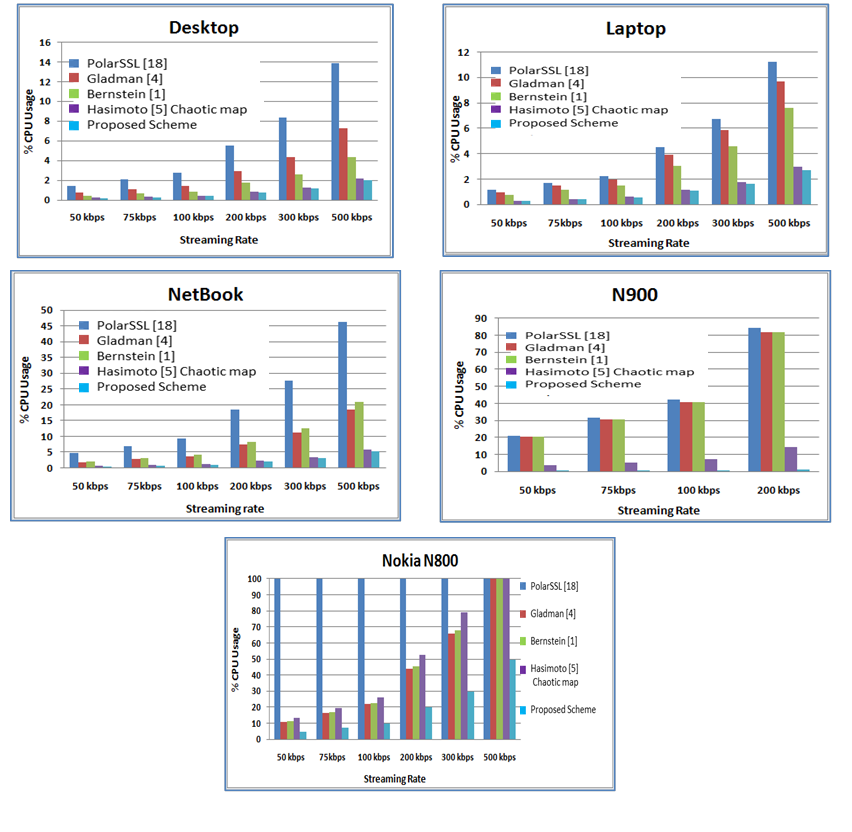
\includegraphics[width=\textwidth]{figure7.png}
\caption{Performance results on different platforms in terms of encryption speed.}
\label{f7}
\end{figure} 

In this section we first analyze the speed and CPU usage on each platform, followed by battery dissipation. Figure~\ref{f7} compares the CPU usage assuming different streaming rates; this means that all implementations are processing the same amount of data over the same period of time. On the desktop, laptop and netbook the proposed scheme is using $\approx$ 15\% less CPU power than the chaotic scheme. But the selective encryption and chaotic encryption are using $\approx$ 150\% less CPU power than all other AES encryption schemes on laptop, desktop and netbook. On Nokia N900 and N800, the proposed scheme is using $\approx$ 2 times less CPU than all other encryption schemes even the chaotic scheme whose CPU usage was close to our scheme. On netbook Gladman's scheme improved its performance in term of CPU usage. OpenSSL CPU usage performance was poor in all platforms.

\begin{figure}[!ht]
\centering
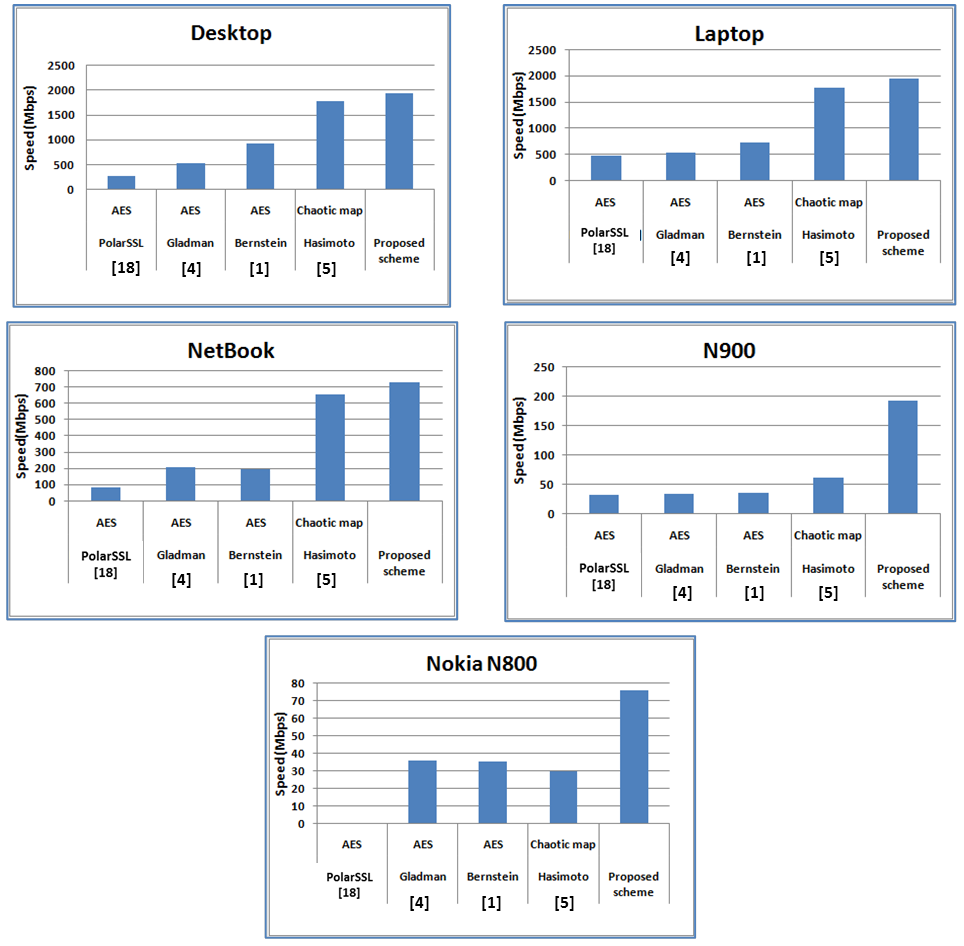
\includegraphics[width=\textwidth]{figure8.png}
\caption{Performance results on different platforms in terms of CPU usage.}
\label{f8}
\end{figure} 

As shown in the graphs of Figure~\ref{f8}, the selective encryption is by far the fastest scheme on all platforms, with an average of $\approx$ 2 ($\approx$ 200\%) times faster than the fastest AES implementation and 15\% faster than the chaotic encryption scheme. Among the AES implementations, Bernstein's implementation obtained the best performance in term of speed, except on the netbook and the N800 device, where Gladman's was the fastest among all the other AES implantations. On N800, the proposed scheme performance was faster than all other Encryption scheme by a factor of $\approx$ 3, and on N900, the proposed scheme enchanted its speed performance to be $\approx$ 5 times faster than all other encryption schemes. This performance improvement is due to the inclusion of a math co-processor in the Nokia N900 architecture (needed for computing chaotic trajectories in Eq.~\ref{ec1}).


Figure~\ref{f9} shows the battery energy consumption on battery operated devices. Figure~\hyperref[f9]{9 a)} shows the performance of encryption schemes in terms of energy usage and the amount of data encrypted within 60 minutes running time. A linear behavior for all implementation is observed with AES implementation having the greatest slopes or energy consumption. For example, Bernstein's implementation encrypts 280 Gbytes of data and consumes over $\approx$ 32 Watt Hour of battery energy on the laptop platform. On the other hand:

\begin{enumerate}
\item The Chaotic scheme encrypts 800 Gbytes of data and consumes the same $\approx$ 32 Watt Hour of the energy on the laptop.
\item The Selective scheme encrypts almost 900 Gbytes of data and consumes the same $\approx$ 32 Watt Hour of the energy on the laptop.
\end{enumerate}

\begin{figure}[!ht]
\centering
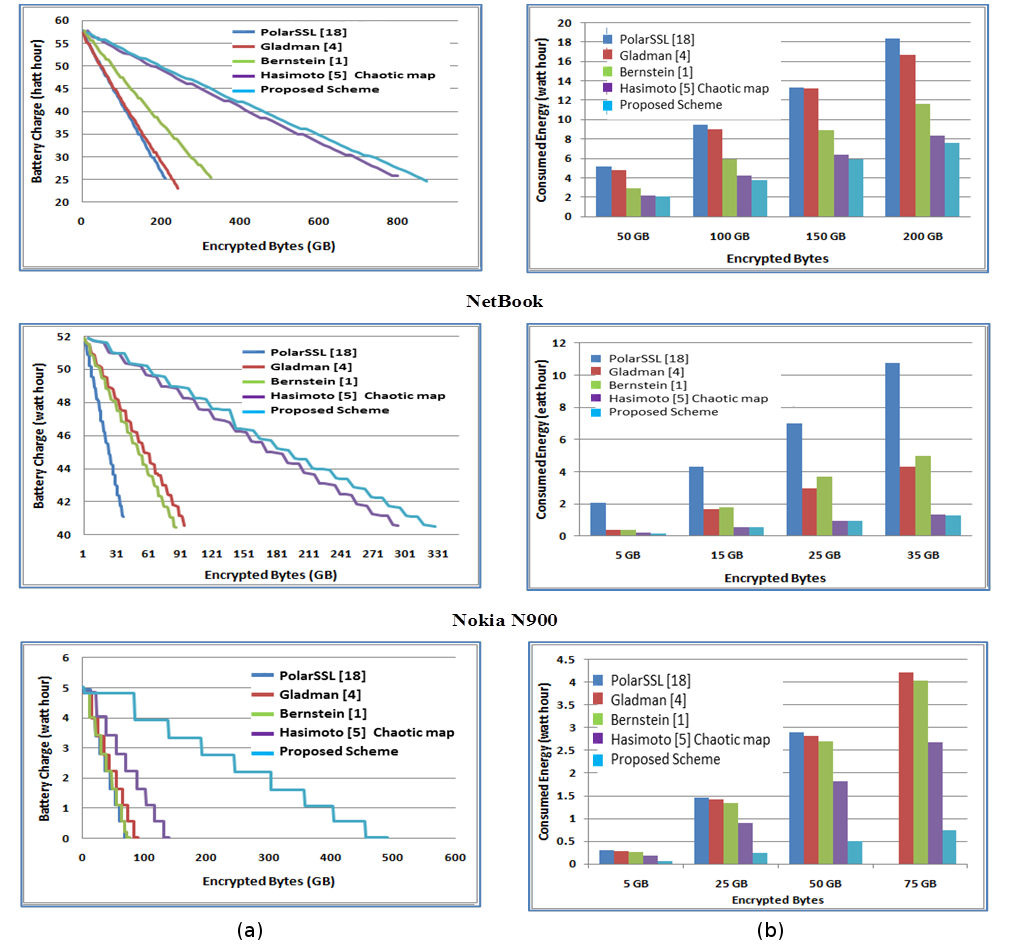
\includegraphics[width=\textwidth]{figure9.png}
\caption{Performance results in terms of energy consumed.}
\label{f9}
\end{figure} 
 
Figure~\hyperref[f9]{9 b)} shows the energy consumed for different data sizes. In Overall, selective encryption can almost process $\approx$ 200\% - $\approx$ 800\% more information with the same energy consumption than all other scheme implementations on all platforms except for chaotic encryption on the laptop, desktop and netbook where the proposed scheme can process $\approx$ 200\% more information with the same energy consumption. 

Figure~\ref{f10} shows the loss of energy resulted by performing the maximum encryption speed of each scheme on the N900 device from full charge state until a complete discharge. As we see from Figure~\ref{f9}, all the schemes follow the same power loss pattern. But in the case of Gladman's scheme and the proposed scheme the battery lives longer even when both are operating in full speed like all others. The reason for this is the power control features of Nokia N900. These results shows that the encryption scheme can be further enhanced by controlling which processor units are used in the encryption.

\begin{figure}[!ht]
\centering
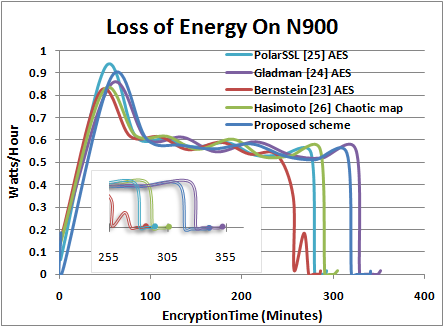
\includegraphics[width=10cm]{figure10.png}
\caption{Loss of Energy on N900.}
\label{f10}
\end{figure} 



In Table~\ref{table4} we compare the proposed scheme with existing work in terms of other parameters and security features.


\begin{table}[!ht]
\centering
\begin{tabular}{p{2.2cm}| c c c c }
\hline 
 \small   \textbf{Scheme}   &
\small  \textbf{Requires}&
\small \textbf{Vulnerable}   &   \textbf{Affects}  &       
\small \textbf{Applicable at} \\ 
& \small \textbf{decoding} & \small \textbf{to plaintext} & \small \textbf{compression}  &  \small \textbf{intermediate}  \\
 &  & \small \textbf{attacks}  &  &\small \textbf{network nodes}  \\ \hline
 	 Shashank~\cite{Khanvilkar2006}  &  Yes  & Yes   &   No     &  No   \\ \hline
 	 Meyer~\cite{Meyer1995}  &  Yes  & No    &   No     &  No   \\ \hline
 	 Spanos~\cite{Spanos1995}  &  Yes  & Yes   &   No     &  No   \\ \hline
 	 Tang~\cite{Tang1996} &  Yes  & No    &   Yes    &  No   \\ \hline
 	 Wu~\cite{Wu2005}  &  Yes  & Yes   &   Yes    &  No   \\ \hline
 	 Wen~\cite{Jiangtao2006} &  Yes  & Yes   &   Yes    &  No   \\ \hline
 	 Proposed  &   No  & No    &   No     &  Yes   \\ 
 	 Scheme  &     &     &        &     \\ \hline
\end{tabular}
\caption{Comparison among different encryption schemes.}
\label{table4}
\end{table}

 
 
\section{Conclusion}
\label{conclusion}

In this paper we have presented a highly scalable encryption scheme for VLC multimedia bit streams that uses computationally efficient chaotic maps based method to generate random numbers. These secure random numbers are then utilized to diffuse correlations among codewords. The proposed scheme is highly robust and scales well in terms of encryption speed and CPU usage with the increase in streaming rate. Our implementation results show over 100\% speedups in execution times across multiple platforms. In terms of CPU usage (and indirectly power usage), the proposed scheme is at least 100\% across platforms. In the work presented in this paper, security is achieved partly due to a robust random number generator. In our future work, we plan to explore codec specific selective schemes and most robust shuffling and diffusion operations that may work on less secure random number generators.


\section*{References}

\bibliography{mybibfile}

\end{document}